% USE \XeLaTeX or \LuaLaTeX please
\documentclass[UTF8]{ctexbeamer}

\usepackage{amsmath}
\usepackage{amssymb}
\usepackage{amsfonts}
\usepackage{multicol}
\usepackage{appendix}

% 参考文献
\usepackage[super]{gbt7714}
% 如果使用的版本为 gbt7714 2.0 (2020年后安装的TeXLive),请移除下一行的注释。
%\bibliographystyle{gbt7714-numerical}

% 设置Beamer主题
%\usetheme[block=fill, sectionpage=none]{metropolis}
\usetheme[block=fill]{metropolis}
\useinnertheme{metropolis}
\usecolortheme{custom}
\useoutertheme{infolines}

\setbeamertemplate{blocks}[rounded][shadow=false]

% \usepackage{authorindex}

% 图片
\usepackage{graphicx}

% 表格
\usepackage{booktabs}
\usepackage{array}

% it used Pygments(a Python lib).
\usepackage{minted}
% pygmentize -L styles
\usemintedstyle{manni}
\usepackage{xcolor}
\definecolor{CodeBackground}{gray}{0.92}
% Use this to replace Fira Code because it's has no Italic.
\usepackage{fontspec}
\setmonofont{Consolas}

% 删除线
\usepackage{ulem}

% 绘图
\usepackage{tikz}
\usetikzlibrary{
  graphs,
  positioning,
  quotes,
  fit,
  calc,
  shapes.geometric,
}
% from https://github.com/muzimuzhi/latex-examples/blob/master/examples/tikz-example-flowchart2.tex
\tikzset{
  meta box/.style={
    draw,
    black,
    very thick,
    text centered
  },
  punkt/.style={
    meta box,
    rectangle,
    rounded corners,
    inner sep=5pt,
    minimum height=2em,
    minimum width=6em,
    align=center,
    text width=6em
  },
  round box/.style={
    meta box,
    circle
  },
  every fit/.style={
    draw,
    thick,
    dashed,
    sec,
    inner sep=6pt
  }
}
\makeatletter
% helper macro
\newcommand\tikz@expand@dimen[2]{\tikzset{minimum #2=#1}}
% tikz styles: adjust min width/height of nodes
\tikzset{
  add dimen/.code 2 args={%
    \pgfkeysgetvalue{/pgf/minimum #1}\tikz@dimen@min
    \expandafter\tikz@expand@dimen\expandafter{\tikz@dimen@min + #2 * 2em}{#1}%
  },
  wider/.style={add dimen={width}{#1}},
  higher/.style={add dimen={height}{#1}},
}
\makeatother
\usepackage{tikz-qtree}

% 题目,作者,学校,日期
\author[GES]{GES\inst{1} \and SYL\inst{1} \and WJX\inst{1} \and WPS\inst{1} \and ZQY\inst{1}}
\title[Xylem]{Xylem}
\subtitle{内容创作平台及管理系统的设计与实现}
\institute[YICAU]{\inst{1} 中国农业大学烟台研究院}
\date{2023 年 11 月 8 日}

\begin{document}

% 设置背景
%\setbeamertemplate{background}{%
%\begin{tikzpicture}\node[inner sep=0pt,outer sep=0pt,opacity=0.14]{\includegraphics[width=\paperwidth,height=\paperwidth,]{assets/}};%
%\end{tikzpicture}%
%}

%% Title
\begin{frame}
\maketitle
\footnote{小组成员按拼音排序。}
\vspace{-55pt}
\end{frame}

%% TOC
\begin{frame}{TOC}
%\setbeamertemplate{section in toc}%[sections numbered]
%\setbeamertemplate{subsection in toc}%[subsections numbered]
\begin{multicols}{2}
\tableofcontents
\end{multicols}
\end{frame}

\section{背景}

\subsection{Where to start?}
%% Origin
\begin{frame}{想法来源}\label{Origin}
\begin{columns}
\begin{column}{0.45\textwidth}
想法的来源是周五(11月3日)在教学楼A区门口看到的小说接龙。

~

\begin{block}{网络平台的接龙小说创作}
知名度较高的包括 SCP 基金会、克苏鲁神话、银河系漫游指南、各类爱好者的 Wiki 等。

甚至跑团也可以理解为通过接龙的形式在创作一部小说。
\end{block}
\end{column}
\begin{column}{0.45\textwidth}
\includegraphics[width=0.85\textwidth, keepaspectratio]{assets/_cgi-bin_mmwebwx-bin_webwxgetmsgimg__&MsgID=1062222612025714843&skey=@crypt_c48cae90_003d4260d6fe495cf9892b2f94ce4065&mmweb_appid=wx_webfilehelper.jpg}\footnotemark[1]
\end{column}
\end{columns}
\footnotetext[1]{拍摄于11月3日下午两点,考虑隐私故对画面内的二维码以及行人进行模糊处理。}
\end{frame}

%% Define scope and domain
\begin{frame}{原型:赛博小说接龙}\label{Prototype}

\begin{tikzpicture}[font=\scriptsize, node font=\scriptsize]\footnotemark[1]
  \node[punkt, wider=1, higher=1]
    (init) {在一个古老的村庄里,当夕阳悄悄…};
  \node[punkt, wider=1, higher=1, right=0.5 of init]
    (follow_1) {陌生的旅行者遇到了一位老人…};
  \node[punkt, wider=1, higher=1, right=0.5 of follow_1]
    (follow_2) {于是他死了};
  \node[punkt, wider=1, higher=1, below=0.5 of follow_2]
    (follow_1_2) {他迅速格挡住了偷袭,进入战斗…};
  \node[punkt, wider=2, higher=1, right=0.5 of follow_2]
    (follow_3) {他在棺材里想:夕阳实在太美了,给我美活了。遂复活。};
  \node[round box, right=0.4 of follow_1_2] (omit_1){\dots};
  \node[round box, below=0.4 of follow_3] (omit_2){\dots};
  \path[arrows={->[scale=1.2]}, thick]
    (init)     edge (follow_1)
    (follow_1) edge (follow_2)
    (follow_1) edge (follow_1_2)
    (follow_2) edge (follow_3)
    (follow_3) edge (omit_2)
    (follow_1_2) edge (omit_1);
  \node[fit=(follow_3),
    label={[sec, anchor=south]north: 妙!}
  ]{};
\end{tikzpicture}

\small

\textbf{目的}:设计一个轻量且易于部署的协同创作平台。

平台在形式上为从生产者向读者传播内容的载体;内容的展现形式遵循树状结构。
而树木的骨架为运输水分的木质部,故起名为 Xylem 。

\footnotetext[1]{以上是对内容的部分文段的展示。cr. CAU 北极星文学社}
\normalsize
\end{frame}

%% Prerequisite
\begin{frame}[fragile]{思路与前置知识}\label{Prerequisite}
\begin{columns}
\begin{column}{0.4\textwidth}
\textbf{开发思路}:产生想法后用最擅长的技术快速出活,反复迭代。

~

涉及到的额外知识:\textbf{假设对课程内容有所了解}
\begin{itemize}
  \item MVC 架构
  \item 一些编程范式(例如面对对象、函数式等)
  \item 基本的 HTML 语法
\end{itemize}

课本之外的专业术语会在对应的页予以解释。
\end{column}
\begin{column}{0.55\textwidth}
\begin{block}{代码实例}
\begin{minted}[
  frame=lines,
  framesep=0.6mm,
  baselinestretch=0.94,
  fontsize=\scriptsize,
  bgcolor=CodeBackground
]{elixir}
defmodule Xylem.Plugs.Auth do
  @behavior Plug

  def init(opts), do: opts

  @doc """
  Invoked when used.
  """
  def call(conn, _opts) do
    conn
    |> fetch_token
    |> query_session
    |> Users.get_by_id
  end
end
\end{minted}
\footnotesize{为方便说明展示会列出部分代码,至多如上所示。}\normalsize  % Return
\end{block}
\end{column}
\end{columns}
\end{frame}

%% About
\begin{frame}[fragile]{关于展示\footnote[1]{用编程语言来描述内容,是技术展示中常见的方法}}\label{About}
\begin{minted}[
  frame=lines,
  framesep=0.6mm,
  baselinestretch=0.98,
  fontsize=\scriptsize,
  bgcolor=CodeBackground,
]{python}
presentation = dict(
    name="Research a MIS",
    required_parts=[
        "background", "analyse requirement", "designing",
        "techstack", "envoirment", "comment"
    ],
    time=lambda t: t <= 5
)

presentation["name"].replace("Research", "Design")
presentation["reference"] = dict(map(
    lambda site: {site, presentation["required_parts"]},
    ["zhihu", "tieba", "Discuz!", "Discord"]
))  # Research many MISs.
presentation["required_parts"] = ["designing", "implementation"]
\end{minted}
\end{frame}
\begin{frame}
\begin{block}{自然语言版本\footnotemark[1]}
\footnotesize
这段Python代码展示了一个项目展示的相关信息和一些操作。
\mintinline{python}|presentation|是一个字典,包含项目展示的相关信息。
\begin{itemize}
  \item \mintinline{python}|"name"|代指项目名称为\mintinline{python}|"Research a MIS"|
  \item \mintinline{python}|"required_parts"|是一个包含字符串的列表,表示项目所需的不同部分
  \item \mintinline{python}|"time"|是一个函数,它接受参数\mintinline{python}|t|,并返回\mintinline{python}|True|如果\mintinline{python}|t|小于等于5,否则返回\mintinline{python}|False|,用于检查展示是否在规定的时间内完成
  \item \mintinline{python}|presentation["name"].replace("Research", "Design")|这一行替换了之前的字符串,使之变成了\mintinline{python}|"Design a MIS"|
  \item \mintinline{python}|presentation["reference"]|是一个通过\mintinline{python}|map|函数构建的字典,将不同的站点名与项目所需的部分关联起来,赋值给该键
  \item 最后将字典中的\mintinline{python}|presentation["required_parts"]|改成了\mintinline{python}|["designing", "implementation"]|
\end{itemize}
需要注意的是,代码中的\mintinline{python}|lambda|函数和\mintinline{python}|map|操作可以使用更明确的方式来构建字典,以提高可读性。
\end{block}
\footnotetext[1]{由 ChatGPT 提供技术支持。}
\normalsize
\end{frame}

\subsection{总结}
\begin{frame}{总结}
\begin{itemize}
  \item 本展示大多以开发者的角度出发,开发一个叫做 Xylem 的系统
  \item 我假定你们对管理信息系统课程的内容有所了解
  \item 对于额外或超纲的内容将以脚注的方式呈现
  \item 除声明外,每节的内容均独立成文
  \item 每节最后都会对本节内容进行总结
\end{itemize}
\end{frame}

\section{设计}

\subsection{战略设计}

\begin{frame}\frametitle{需求与核心功能分析}
赛博接龙小说的问题:
\begin{itemize}
  \item 世界观不连贯
  \item 捣蛋鬼来捣蛋(互联网平台的通病)\footnote[1]{在互联网,没人知道你是一条狗。}
  \item 前期作者的作品对后续作者的发挥带来限制
  \item 接龙创作的线性内容形式不利于从群体中选出最好的
\end{itemize}

\textbf{解决方案}:以内容为主;除了发起人声明外默认可以随意创作(从任何地方开始)。

\end{frame}

\subsection{消化知识与细化概念}

\begin{frame}{用户}
按照 Xylem 的设计理念,平台将大多数用户定义为内容生产者以及读者。
其中,前者负责生产内容,而后者对内容进行评价。
因此用户管理规范相比其他的系统有较大的差异。

其中包括用户的注册与版权问题,因为内网的情况前者不需要邮件,如果用户绑定邮件可以选择内容的版权许可证,否则默认公有领域。
\begin{block}{版权争端}
早期知乎的知识产权协议近乎霸王条款:
「对于用户发表到知乎上的任何内容,用户同意知乎在全世界范围内具有免费的、永久性的、不可撤销的、排他性的和完全再许可权的权利和许可,以行使和保护与内容相关的全部著作权。」

后期知乎更新了著作权协议,可以在禁止转载到可以转载二者之间选择。
\end{block}
\end{frame}

\begin{frame}{协同创作的实现}
%\begin{columns}
%\begin{column}{0.5\textwidth}
\emph{Scenario i}: \textbf{接龙写作}:

以句子或段落为基本单位,用户均可对公开故事进行续写(可以编辑自己写的部分),并且可以对其他作品表态或评论。
(类似于论坛但可以随意接龙,详见最后一节)

%\end{column}
%\begin{column}{0.5\textwidth}
\emph{Scenario ii}: \textbf{协同创作}:

在同一世界观下共同创作(类似于Wiki,但也可以在前者的机制下实现)

%TODO: 用户组(详见内容管理)
%TODO: 状态:不可见/可见

\emph{Scenario iii}: \textbf{跑团}
%\end{column}
%\end{columns}
\end{frame}

\begin{frame}{文字创作}
在形式上与论坛有相同但是存在差别,故使用新的名称\footnote[1]{部分内容参考了 FimTale 的用户手册},例如:

\begin{itemize}
  \item 全站点的管理层 $\rightarrow$ 管理团队
  \item 楼主/PO主 $\rightarrow$ 发起人
  \item 帖子 $\rightarrow$ 故事
  \item 跟帖 $\rightarrow$ 续写
  \item 草稿箱外每次提交的记录 $\rightarrow$ 记录
\end{itemize}

\begin{block}{DDD 的模式:通用语言(Ubiquitous Language)}
%确保开发者队伍的纯洁性与先进性要从对齐思想开始。
%开发者要有统一的大局意识,在大局中思考、在大局下行动。
%话往一处讲,劲往一处使。协创共进,更快更好的完成系统的开发。
通用语言是领域驱动设计(DDD)开发中的使用的语言(包括术语以及描述方式),用于确保开发团队和业务团队之间使用相同的术语和概念,以便更好地理解和沟通领域需求,从而提高软件开发的质量和效率。
% 使用一致的语言有助于消除沟通障碍,促进协作,使整个团队更好地理解和共享领域知识。
\end{block}
\end{frame}

\begin{frame}{内容的格式与改动}
内容的格式采用 Markdown 或 BBCode \footnote[1]{以上均属于轻量级标记语言,使用简单的记号来对内容的格式进行标识。},采用句子或分段为分割单位,选择什么取决于用户的要求。

Xylem 给予用户对内容的修改权力,同时也允许用户回滚到之前的某次修改。

对于表态的排名,对根据修改内容站之前内容的比重进行加权处理,以作为展现层的排名的依据。

当某内容被删除时,后续内容会根据被删除的原因而不可添加内容/设为不可见/标记“上游信息被删除,可能无法保证内容连贯”的措施等处理。
\end{frame}

%\begin{frame}{不涉及正文的评价交流}
%TODO: \textbf{他山之石:FimTale}
%\end{frame}

\subsection{管理}

\begin{frame}{内容管理}
Xylem 的原则是「为所涉及的内容负责」,但考虑到可能有用户无法遵循该原则,因此需要引入管理机制。

Xylem 的内容管理权限将从维护者到发起人;从发起人到所发起的故事(主要为控制可见度);用户则对其所发表的内容负责。

处理手段包括:
\small
\begin{itemize}
  \item 向用户发送警告
  \item 内容不能被表态或评论
  \item 删除内容
  \item 删除内容并冻结账号
  \item 封禁 IP ,将日志上报学校(Xylem 在内网部署)
\end{itemize}
\normalsize
\end{frame}

\begin{frame}{面向维护者的功能}
面向维护者的功能主要包括控制台(dashboard)以及统计(statistics)。

\small
功能包括:\begin{itemize}
  \item 系统状态
  \item 服务列举与配置\footnote[1]{参见最后一节「二次开发」。}
  \item 依赖配置与占用资源
  \item 用户统计
  \item 故事统计
  \item 推送设定
\end{itemize}
\normalsize
\end{frame}

%\begin{frame}{用户管理与准入门槛}
%主要是上者「协同创作的实现」的\emph{Scenario ii}。
%故事发起人负责的业务,作为防捣乱(后者)的一部分。
%\end{frame}

%\begin{frame}{「反熊」}
%确保操作账号的是人类;
%TODO: 不同层级
%访问层面;账号层面(业务);内容层面(故事)
%\end{frame}

\subsection{总结}
\begin{frame}{总结}
\begin{itemize}
  \item 为了专注于创作,以内容作为第一出发点而非用户
  \item 内容以多种形式表达,主要是类似论坛的发帖回帖制,可能也会提供可以即时通信的聊天室
  \item 接龙形式的内容只有部分反响较好者可以在帖子/平台的时间线被所有人访问,但是所有未被删除的内容均可通过链接直接访问
  \item 除用户同时在平台以及社交网站声明外,所生产内容的版权默认属于公共领域,对于没有版权声明且可访问的内容,提供导出功能
  \item 内容管理的权限通过管理团队到对应故事的发起人、发起人到参与续写的用户的多层赋权实现
  \item 用户可以对平台内的公共领域的内容做出回应、评论,其能够影响展示的排名(存在不同的排名机制),也是被导出的一部分
\end{itemize}
\end{frame}

\section{实现}

\subsection{技术选择}

\begin{frame}{战术设计}
\textbf{一句话}:关于如何实现软件系统的具体细节和技术方案的计划和决策。

包括但不限于架构选择、编程语言选择、代码规范确定、代码审查机制确定、测试规范等等。

\begin{block}{MVC架构}
MVC架构(Model-View-Controller)是一种用于组织和分离应用程序代码的设计模式。
在MVC中,模型(Model)负责管理应用程序的数据和业务逻辑\footnotemark[1],
视图(View)负责呈现数据和用户界面,而控制器(Controller)充当数据和用户界面之间的中介,接收用户输入并协调模型和视图之间的交互。
该架构使代码更易于维护和扩展,因为不同部分之间的职责被清晰划分,允许独立地修改和更新每个部分而不会影响整个应用程序。
\end{block}
\footnotetext[1]{对于业务逻辑应该放到哪里,不同的MVC框架有不同的处理方案}
\end{frame}

\begin{frame}{运行环境与技术栈}
\begin{columns}
\begin{column}{0.44\textwidth}
路线:快速开发、方便部署/跟随潮流、挑战新奇。
\begin{block}{技术栈\footnotemark[1]}
包括开发所用到的编程语言、框架、数据库、操作系统、开发工具、版本控制系统等。

可以以数据架构图的形式存在,也可以以组件首字母缩写表示。
\end{block}
\end{column}
\begin{column}{0.52\textwidth}
\textbf{他山之石:其他论坛的技术选择}

\begin{itemize}
  \item \emph{NodeBB}~基于 Node.js 开发
  \item \emph{Discuz!}~基于 PHP 开发
  \item \emph{discourse}~基于 RoR 开发,只能在 Docker 上运行
  \item \emph{discord}~基于 Elixir 开发,维护人数少并发能力强,但函数式编程存在门槛
\end{itemize}
\end{column}
\end{columns}
选择的依据更多的取决于项目需求以及你所有的技能树。

Xylem 打算选什么?
根据\href{https://ges233.github.io/about}{所会技术},
选择 \href{https://www.python.org/}{Python}/\href{https://sanic.dev/}{Sanic}/\href{https://picocss.com}{PicoCSS}/\href{https://alpinejs.dev/}{Alpine.js} 。
(运行环境:Unbuntu/Windows + SQLite + Redis(Optional))

\footnotetext[1]{把一项产品所用到的一系列相互关联的技术和工具堆起来就叫做技术栈。}
\end{frame}

\begin{frame}{解(chao)剖(xi)开源信息系统的方法/流程}
(假设已经做好背调)

\begin{itemize}
  \item 本地部署,探索系统的功能
  \item 查看包括用户手册、开发文档、API文档等的项目文档,了解基本信息
  \item 根据配置文件以及文件结构,了解项目的各部分
  \item 对数据模型进行研究,包括数据表以及各层次的数据
  \item 结合功能与数据,阅读源代码对功能的实现方式进行研究
\end{itemize}
\end{frame}

\subsection{建立项目}

\begin{frame}[fragile]{项目的组织与配置}\label{Orgnise}
\begin{columns}

\begin{column}{0.5\textwidth}
\begin{minted}[
  frame=lines,
  framesep=0.6mm,
  baselinestretch=0.84,
  fontsize=\scriptsize,
  bgcolor=CodeBackground
]{text}
ROOT
+-config/
+-instance/
+-tests/
+-priv/  # Inspired by Phoenix
| +-assets/
| +-template/
| +-pics/
+-xylem/
| +-adapter/
| +-helpers/
| +-infra/
| +-services/
| +-xylem_core/
| +-xylem_domain/
| +-xylem_web/
+-run.bat
+-README.txt
\end{minted}

项目采用了整洁架构(Clean Architecture)的变体。
\end{column}
\begin{column}{0.4\textwidth}
\begin{block}{库、框架与架构的区别}
库是一系列预先编写好的代码集合,供开发者在编程中调用。

框架是会介入编程人员工作的库,负责具体实现程序员书写的业务,能够接管程序的控制流。

架构是高度抽象的需求,是系统中的不变量。随着业务的抽象在不同的层级有不同的含义。
\end{block}
\end{column}

\end{columns}
\end{frame}

\subsection{数据与关系}

%% 抽象的索引,真实的集合
\begin{frame}{数据表关系}
\includegraphics[height=0.8\textheight, keepaspectratio]{assets/Xylem_relationship.png}\footnotemark[1]
\footnotetext[1]{跑团部分过于复杂,不予考虑}
\end{frame}

\begin{frame}[fragile]{树形关系的实现}
\begin{columns}
\begin{column}{0.35\textwidth}
对内容的读写符合以下规则:

查看某些有价值或令人忍俊不禁的 $\gg$ 添加 \textgreater 查看所有的

\begin{block}{嵌套集}
嵌套集是一种用于组织和表示层次结构数据的数据库模型。
核心是使用两个字段来表示节点在树中的位置:左边界(lft)和右边界(rgt)。
\end{block}
\end{column}
\begin{column}{0.65\textwidth}
\begin{minted}[
  frame=lines,
  framesep=0.6mm,
  baselinestretch=0.98,
  fontsize=\scriptsize,
  bgcolor=CodeBackground,
  breaklines
]{sql}
-- Use comment as example.
CREATE TABLE comments(
  id INTEGER PRIMARY KEY,
  content TEXT,
  root_id INTEGER FOREIGN KEY,
  lft INTEGER,
  rgt INTEGER,
  create_at DATETIME,
  likes INTEGER,
  -- Optional
  depth INTEGER,
);

-- Insert comments.
INSERT comments VALUES
  (1, "给我笑拥了", 1, 1, 2, NOW(), 0, 1)
  (2, "我申气了", 1, 3, 4, NOW(), 0, 1)
  (3, "好好好", 1, 5, 6, NOW(), 0, 1)
  (4, "强而有力,强而有力啊", 1, 7, 8, NOW(), 0, 1);
\end{minted}
\end{column}
\end{columns}
\end{frame}

\begin{frame}[fragile]{树形关系的实现(简单查询)}
\begin{columns}
\begin{column}{0.45\textwidth}
例如:返回【一条】已知 id 的评论。

~

\includegraphics[width=0.9\textwidth, keepaspectratio]{assets/comment_0.png}

\end{column}
\begin{column}{0.5\textwidth}
\begin{minted}[
  frame=lines,
  framesep=0.6mm,
  baselinestretch=0.98,
  fontsize=\scriptsize,
  bgcolor=CodeBackground,
  breaklines,
]{sql}
-- Read comment.
SELECT (
  comments.id,
  comments.root_id,
  comments.content,
  comments.create_at
) FROM comments WHERE (
  comments.root_id = 
  AND comments.id = 4
);
\end{minted}
~

将返回:
\scriptsize
\mintinline[breaklines]{text}|4, 1, "强而有力,强而有力啊", 2023/11/08T10:25:03|
\normalsize

\end{column}
\end{columns}
\end{frame}

\begin{frame}[fragile]{树形关系的实现(插入)}
\begin{columns}
\begin{column}{0.5\textwidth}
插入一条新评论\footnotemark[1]。

~

\includegraphics[width=0.9\textwidth, keepaspectratio]{assets/comment_init.png}
\end{column}
\begin{column}{0.45\textwidth}
\begin{minted}[
  frame=lines,
  framesep=0.6mm,
  baselinestretch=0.98,
  fontsize=\scriptsize,
  bgcolor=CodeBackground,
  breaklines,
]{sql}
INSERT INTO comments VALUES(
  5, "会读书的拟人最美丽",
  1, 2, 3, NOW(),
  0, 2
);

UPDATE comments SET
  lft = (
    CASE WHEN lft >= 3 THEN lft + 2 ELSE lft END
  ), rgt = (
    CASE WHEN rgt >= 2 THEN rgt + 2 ELSE rgt END
  )
WHERE root_id = 1;
\end{minted}
\end{column}
\end{columns}

\footnotetext[1]{绘图只有一部分。}
\end{frame}

\begin{frame}[fragile]{树形关系的实现(复杂查询)}
\begin{columns}
\begin{column}{0.5\textwidth}
查询某评论下【所有】的子评论。

~

\includegraphics[width=0.9\textwidth, keepaspectratio]{assets/insert_comment_after_update.png}
\end{column}
\begin{column}{0.45\textwidth}
\begin{minted}[
  frame=lines,
  framesep=0.6mm,
  baselinestretch=0.98,
  fontsize=\scriptsize,
  bgcolor=CodeBackground,
  breaklines,
]{sql}
SELECT (
  comments.id,
  comments.root_id,
  comments.content,
  comments.create_at,
  comments.depth
) FROM comments WHERE (
  comments.lft >= 1 AND comments.rgt <=6
);
\end{minted}
\end{column}
\end{columns}
\end{frame}

\subsection{功能与服务的实现}

\begin{frame}{用户邀请、注册与登录}
\begin{columns}
\begin{column}{0.7\textwidth}
邀请与注册:
\end{column}
\begin{column}{0.3\textwidth}
登录:
\end{column}
\end{columns}

~

\begin{tikzpicture}[font=\scriptsize, node font=\scriptsize]
  \node[draw, rounded corners]    (init) {开始邀请};
  \node[draw, below=0.3 of init] (active) {申请邀请码};
  \node[draw, diamond, aspect=2, below=0.3 of active] (valid) {用户状态正常?};
  \node[draw, left=10pt of valid]  (invalid) {拒绝};
  \node[draw, below=0.3 of valid]  (generate) {生成邀请码};
  \node[draw, below=0.3 of generate] (record) {记录用户};
  \node[draw, rounded corners, below=0.3 of record] (end) {结束};

  \draw[->] (init) -- (active);
  \draw[->] (active) -- (valid);
  \draw[->] (valid) -- (invalid);
  \draw[->] (valid) -- (generate);
  \draw[->] (generate) -- (record);
  \draw[->] (record) -- (end);

  %% Register
  \node[draw, rounded corners, right=1.4 of init] (reg) {开始注册};
  \node[draw, diamond, aspect=2, below=0.5 of reg] (valid_) {验证邀请码/昵称};
  \node[draw, right=10pt of valid_] (failed) {出现错误};
  \node[draw, below=0.3 of valid_] (add) {记录用户(用户表;邀请表)};
  \node[draw, rounded corners, above=0.5 of failed] (err_end) {结束};

  \graph{
    (reg) -> (valid_) -> (add) -> (end);
    (valid_) -> (failed) -> (err_end);
  };

  \node[draw, rounded corners, right=0.5 of failed] (signin) {登录};
  \node[draw, diamond, aspect=2, below=0.5 of signin] (check) {有昵称密码匹配的用户?};
  \node[draw, below=0.5 of check] (login) {返回内容,成功};

  \graph{
    (signin) -> (check) -> (failed) -> (err_end);
    (check) -> (login) -> (end);
  };
\end{tikzpicture}
\end{frame}

\begin{frame}{创建故事}
\footnotesize
欢迎旅行者,接下来等着你的居然是\dots
\begin{center}
\begin{tikzpicture}[font=\scriptsize, node font=\scriptsize]
  \node[draw, rounded corners]    (init) {开始};
  \node[draw, below=0.5 of init]  (advocate) {向管理团队申请};
  \node[draw, diamond, aspect=3, below=0.5 of advocate] (filter) {审查};
  \node[draw, below=0.5 of filter]  (edit) {改进};
  \node[draw, left=0.5 of filter]  (refuse) {拒绝};
  \node[draw, right=0.5 of filter] (pass) {通过};
  \node[draw, rounded corners, below=0.5 of edit]  (end) {结束};

  \graph{
    (init) -> (advocate) -> (filter);
    (filter) -> (edit) -> (filter);
    (filter) -> (refuse) -> (end);
    (filter) -> (pass) -> (end);
  };
\end{tikzpicture}
\end{center}
\normalsize
\end{frame}

\begin{frame}{创建并修改内容}
\includegraphics[width=0.9\textwidth, keepaspectratio]{assets/tikzit_image0.png}\footnote[1]{由 TikZit 生成。}
\end{frame}

\begin{frame}{对内容的评价体系}
我们将内容看成有$n$个节点的树$\mathrm{T}$,其中值就是对单个节点的评价。

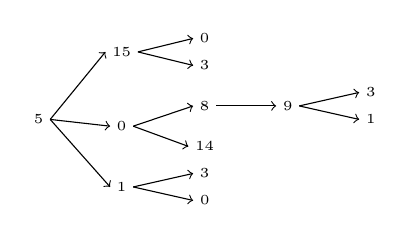
\begin{tikzpicture}[font=\tiny, node font=\tiny, grow=right,->]
  \Tree[.5 [ .1 [ .0 ] [ .3 ] ] [ .0 [ .14 ] [ .8 [ .9 [ .1 ] [ .3 ] ] ] ] [ .15 [ .3 ] [ .0 ] ]]
\end{tikzpicture}

% 选择最受欢迎的序列 $\mathrm{T}_{Seq = \{i, j, k, \dots\}}$ 就可以看成:
%在 $\mathrm{T}$ 中选择特定满足任意 $i \neq j $ 的 $i, j \in Seq$ 都有
%$\mathrm{T}_{Seq[i]}~in~\mathrm{T}_{Seq[j]}$ 或 $\mathrm{T}_{Seq[j]}~in~\mathrm{T}_{Seq[i]}$ 的
%$Seq \in \mathbb{N}$ 使得 $\sum \mathrm{T}_{Seq}$ 或 $\sum \frac{\mathrm{T}_{Seq}}{n}$ 最大。

对于没有子节点的节点(还没人回复的某内容) $T_i$ 来讲,
该讨论串(从最开始的内容到该回复的所有内容)的值就是可计算的。

对内容的评价就取决于该值与该节点的深度。

计算的方式可以是累加,也可以先通过算法进行修正再累加。
%TODO: 排名算法
\end{frame}

\begin{frame}{牛顿冷却定律:对评价的排序算法的实现}
将内容的「热度」看成自然的温度,运用自然科学的方法解决问题:

\begin{align}
  T' (t) &= -k \Delta T \\
  T' (t) &= -k (T - H) \\
  \frac{\mathrm{d}T}{\mathrm{d}t} &= -k (T - H) \\
  \frac{\mathrm{d}T}{T - H} &= -k \mathrm{d}t
\end{align}

取积分,得:

$$\int \frac{1}{T - H} \mathrm{d}T = -k \int \mathrm{d}t$$
\end{frame}

\begin{frame}{牛顿冷却定律(续)}
可得:

$$\ln (T - H) = -kt + C$$

两边同时指数,得:

%\begin{align}
%e^{\ln (T - H)} &= e^{-kt + C} \\
$$T - H = C e^{-kt}$$
%\end{align}

在时间 $t_0$ 存在已知的 $T_0$ ,有:

\begin{align}
T_0 - H &= C e^{-kt_0} \\
C &= (T_0 - H) e^{kt_0}
\end{align}
\end{frame}

\begin{frame}{牛顿冷却定律(续)}
将其代入,可得:

$$
T = (T_0 - H) e^{k(t_0 - t)} + H
$$

没有热度时 $H = 0$ ,有:

$$
T = T_0 e ^{-k(t - t_0)}
$$

\small
其中 $k$ 为大于零的常数,$T_0$ 为 $t_0$ 时的温度。
\normalsize
\end{frame}

\begin{frame}[fragile]{牛顿冷却定律的实现}
\begin{minted}[
  frame=lines,
  framesep=0.6mm,
  baselinestretch=0.98,
  fontsize=\scriptsize,
  bgcolor=CodeBackground,
  breaklines
]{python}
import math

def newtons_law_of_cool(
    T_prev: int | float, delta: float, k: float
) -> float:
    return T_prev * math.exp(-k * delta)

>>> print(newtons_law_of_cool(100, 0.5, 1))
60.653065971263345
\end{minted}
\end{frame}

\begin{frame}{类聊天室的设计}
\begin{columns}
\begin{column}{0.4\textwidth}
\begin{block}{他山之石:TRPG Engine}
TRPG Engine 是一款帮助用户更加方便跑团的即时通信软件。
该项目的定位是帮助用户更快很好的进行沟通与交互的引擎,也让主持人将精力专注于剧情、场景上。

在提供即时通信服务的基础上提供了一站式跑团(包括车卡、骰子等)的服务。
\end{block}
\end{column}
\begin{column}{0.5\textwidth}
在前端界面上和 Discord 类似(都是基于 React 进行开发)。

TRPG Engine 的实时消息推送使用 WebSocket 实现。
基于 Socket.io 框架进行开发,该服务被应用注册到中间件(Middleware)\footnotemark[1]。

由于源代码中数据库的迁移记录有近百条,数据库共计几十张表以及一千多行列。
加之没有 Node.js 的开发经验,故放弃深入研究。
\end{column}
\end{columns}
\footnotetext[1]{中间件是计算机软件中的「传话者」,协同其他组件相互协调。}
\end{frame}

\subsection{开发与发布}

\begin{frame}{网络安全}
业务上的安全:
\begin{itemize}
  \item 用户登录解决方案(Session Cookie)
  \item 用户的密码混淆
  \item 访问控制
  \item 发帖控制
\end{itemize}

基层设施的安全:
\begin{itemize}
  \item 对来自客户的请求频次设置阈值(反脚本)
  \item XSS、CRSF
  \item 反向代理
\end{itemize}
\end{frame}

\begin{frame}[fragile]{Pluggable Xylem:二次开发与可插拔模块设计}
项目将所有的功能都写到了 /xylem/services/ 内,并通过依赖注入\footnote[1]{依赖注入允许你将一个对象的依赖关系(通常是其他对象或服务)从外部传递给该对象,而不是在对象内部硬编码这些依赖关系。这使得代码更加松散耦合、可维护和可测试。}
(演示见下)的方式被注册到了应用中。
因此二次开发仅需要将功能封装成服务,注册到中间件或路由函数即可。
\begin{columns}
\begin{column}{0.55\textwidth}
\begin{minted}[
  frame=lines,
  framesep=0.6mm,
  baselinestretch=0.98,
  fontsize=\scriptsize,
  bgcolor=CodeBackground,
  breaklines
]{python}
class UserAnalyseService(XyService):
    orinted: [xylem.xylem_core.user, xylem.xylem_core.content_base]

    def __fetch__(self):
        pass
    
    ...

\end{minted}
\end{column}
\begin{column}{0.45\textwidth}
\begin{minted}[
  frame=lines,
  framesep=0.6mm,
  baselinestretch=0.98,
  fontsize=\scriptsize,
  bgcolor=CodeBackground,
  breaklines
]{python}
# In handler module.

async def write(
    request: Request, service: UserAnalyseService
) -> HTTPResponse:

    ...
\end{minted}
\end{column}
\end{columns}
% \footnote[2]{依赖注入之实例。}
\end{frame}

\begin{frame}{软件生命周期与交付}
版本号按照 ~\mintinline{text}|{major}.{minor}.{micro}|~ 的格式。
由于业务需求相对稳定,因此在正式版(v1.0.0)发布后主要以维护为主。

在开发完成部署后需要注意的方面:
\begin{itemize}
  \item 生产环境与开发环境
  \item 应用的配置
\end{itemize}

\begin{block}{部署}
考虑到使用场景,最好的方法是把 Xylem 打包成一个可执行的应用文件。
除此之外,额外需要的程序仅包括 SQLite。

当然,如果需要长期运行的话,也支持基于 Docker 的部署服务。
\end{block}
\end{frame}

\subsection{总结}
\begin{frame}{总结}
\begin{itemize}
  \item \sout{从实现细节描述了调研系统的思路与方法}
  \item \sout{介绍了多种实现功能需要的算法}
  % \item \sout{介绍了}
  \item 本节没什么要总结的
\end{itemize}
\end{frame}

\appendix

\section{附录}

%\begin{frame}[allowframebreaks]{参考文献}
%\bibliography{Slides}
%\end{frame}

\begin{frame}{媒体资源}

\begin{itemize}
    \item \textbf{Slides}: \textbf{\LaTeX{}} + \textbf{Beamer} + \textbf{\textsc{metropolis}}
    \item \textbf{\sout{完颜慧德老师}小说接龙的照片}: 拍摄
    \item \textbf{评论的节点图}: 使用免费软件 draw.io 绘制
    \item \textbf{关系图}: 使用 dbdiagram.io 的服务生成
\end{itemize}

\end{frame}

\begin{frame}[label=end, standout]
感谢大家收听!
\end{frame}

\end{document}
